
\begin{enumerate}
    \item If the process on one mole of monatomic ideal gas is as shown in the TV-diagram with \( P_0 V_0 = \frac{1}{3} RT_0 \), the correct match is,
        \begin{tasks}(2)
            \task \(I \rightarrow P, II \rightarrow R, III \rightarrow T, IV \rightarrow S\)
            \task \(I \rightarrow P, II \rightarrow T, III \rightarrow Q, IV \rightarrow T\)
            \task \(I \rightarrow P, II \rightarrow R, III \rightarrow T, IV \rightarrow P\)
            \task \(I \rightarrow S, II \rightarrow T, III \rightarrow Q, IV \rightarrow U\)
        \end{tasks}
    \item[\textbf{Diagram:}]
        \begin{center}
            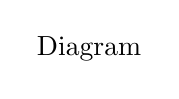
\begin{tikzpicture}
                \node {Diagram};
            \end{tikzpicture}
        \end{center}
\end{enumerate}
